\documentclass[11pt,a4paper]{article}
\usepackage[spanish,es-nodecimaldot]{babel}	% Utilizar español
\usepackage[utf8]{inputenc}					% Caracteres UTF-8
\usepackage{graphicx}						% Imagenes
\PassOptionsToPackage{hyphens}{url}
\usepackage[hidelinks]{hyperref}			% Poner enlaces sin marcarlos en rojo
\usepackage{fancyhdr}						% Modificar encabezados y pies de pagina
\usepackage{float}							% Insertar figuras
\usepackage[textwidth=390pt]{geometry}		% Anchura de la pagina
\usepackage[nottoc]{tocbibind}				% Referencias (no incluir num pagina indice en Indice)
\usepackage{enumitem}						% Permitir enumerate con distintos simbolos
\usepackage[T1]{fontenc}					% Usar textsc en sections
\usepackage{amsmath}						% Símbolos matemáticos
\usepackage{natbib}

% Comando para poner el nombre de la asignatura
\newcommand{\asignatura}{Visión por Computador}
\newcommand{\autor}{Vladislav Nikolov Vasilev}
\newcommand{\titulo}{Trabajo 2}
\newcommand{\subtitulo}{Cuestiones de teoría}

\newcommand{\answer}{\noindent\textbf{Solución}}
\newcommand{\question}[1]{\noindent\textbf{#1}}
\newcommand{\nonumsection}[1]{\section*{#1}\addcontentsline{toc}{section}{#1}}

% Configuracion de encabezados y pies de pagina
\pagestyle{fancy}
\lhead{\autor{}}
\rhead{\asignatura{}}
\lfoot{Grado en Ingeniería Informática}
\cfoot{}
\rfoot{\thepage}
\renewcommand{\headrulewidth}{0.4pt}		% Linea cabeza de pagina
\renewcommand{\footrulewidth}{0.4pt}		% Linea pie de pagina

\begin{document}
\pagenumbering{gobble}

% Pagina de titulo
\begin{titlepage}

\begin{minipage}{\textwidth}

\centering

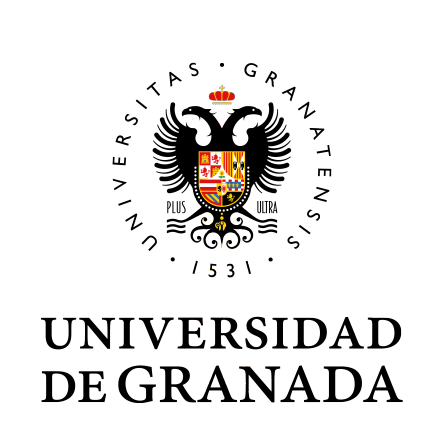
\includegraphics[scale=0.5]{img/ugr.png}\\

\textsc{\Large \asignatura{}\\[0.2cm]}
\textsc{GRADO EN INGENIERÍA INFORMÁTICA}\\[1cm]

\noindent\rule[-1ex]{\textwidth}{1pt}\\[1.5ex]
\textsc{{\Huge \titulo\\[0.5ex]}}
\textsc{{\Large \subtitulo\\}}
\noindent\rule[-1ex]{\textwidth}{2pt}\\[3.5ex]

\end{minipage}

\vspace{0.5cm}

\begin{minipage}{\textwidth}

\centering

\textbf{Autor}\\ {\autor{}}\\[2.5ex]
\textbf{Rama}\\ {Computación y Sistemas Inteligentes}\\[2.5ex]
\vspace{0.3cm}


\includegraphics[scale=0.3]{img/etsiit.jpeg}

\vspace{0.7cm}
\textsc{Escuela Técnica Superior de Ingenierías Informática y de Telecomunicación}\\
\vspace{1cm}
\textsc{Curso 2019-2020}
\end{minipage}
\end{titlepage}

\pagenumbering{arabic}
\tableofcontents
\thispagestyle{empty}				% No usar estilo en la pagina de indice

\newpage

\setlength{\parskip}{1em}

\nonumsection{Ejercicio 1}

\question{Identifique las semejanzas y diferencias entre los problemas
de: a) clasificación de imágenes; b) detección de objetos: c)
segmentación de imágenes; d) segmentación de instancias.}

\answer

La clasificación de imágenes consiste en asignar una clase a una imagen
de entrada. La detección de objetos permite determinar qué objetos hay
en una imagen y localizándolos dentre de ésta, de forma que se muestra una
\textit{bounding box} a su alrededory se identifica
de qué clase son los objetos detectados. La segmentación de imágenes consiste
en clasificar cada píxel de una imagen, asignándole una u otra clase. La
segmentación de instancias permite distinguir entre las distintas instancias
de los objetos encontrados dentro de la imagen, de forma que, a pesar de que
puedan pertenecer a la misma clase, sean tratados como entidades diferentes de
una misma clase.

Como se puede ver, cada problema tiene sus peculiaridades, ya que en cada
uno se persigue resolver cosas diferentea. Sin embargo, existen ciertas
similitudes entre ellos. Por ejemplo, tanto en la clasificación de imágenes como
en la detección de objetos se predice una clase (en el primer caso, es el
problema principal, mientras que en el segundo se predice de qué tipo
es el objeto detectado dentro de los tipos conocidos). La segmentación
de imágenes parece una mezcla de la detección de objetos y clasificación,
ya que se trata de una clasificación de más bajo nivel (píxel a píxel), y en
dicho proceso se detectan objetos de distintas clases. La segmentación
de instancias es un paso más allá de la detección de objetos, ya que permite
detectar objetos dentro de la imagen al mismo nivel que la segmentación de imágenes
(a nivel de píxel) y permite distinguir entre las distintas instancias de
los objetos de una misma clase. Por tanto, es una sofisticación de la
detección de objetos.

\nonumsection{Ejercicio 2}

\question{¿Cuál es la técnica de búsqueda estándar para la detección de
objetos en una imagen? Identifique pros y contras de la misma e
indique posibles soluciones para estos últimos.}

\answer

La técnica estándar para detectar objetos en imágenes es la \textbf{\textit{sliding window}}
o \textbf{ventana deslizante}. Esta técnica consiste en pasar un rectángulo
de dimensiones fijas por la imagen obteniendo una ventana. Dicha ventana es
pasada luego a un clasificador, el cuál predice si está o no el objeto a detectar
dentro de esa ventana. Ese clasificador debe haber sido entrenado previamente
para detectar objetos de la clase a buscar.

La principal ventaja es que una técnica que descompone un problema
relativamente complejo, que es la detección de objetos dentro de imágenes,
en un problema más simple de clasificación (decir si está o no el objeto).
Además es una técnica conceptualmente sencilla, con lo cuál es relativamente
fácil de implementar. Sin embargo, como toda técnica, tiene sus desventajas:

\begin{itemize}[label=\textbullet]
  \item \textbf{Coste computacional alto.} Esta técnica es costosa, ya que
  se deben clasificar muchas ventanas de una imagen, y además, los desplazamientos
  de la ventana por la imagen no pueden ser pequeños, ya que si lo fuesen, la técnica
  sería totalmente inviable, porque se tardaría demasiado tiempo en procesar la imagen
  completa.
  \item \textbf{Detectar objetos de diferentes tamaños.} Este es uno de los
  problemas más básicos. Si el tamaño de la ventana es demasiado pequeño, a
  lo mejor se pierden algunos de los objetos de la imagen, ya que son demasiado
  grandes como para ser detectados. Para ello, se puede o bien pasar
  ventanas de distinto tamaño por la imagen, o bien se puede construir un
  espacio de escalas de la imagen, utilizando por ejemplo la pirámide Gaussiana,
  y pasar la misma ventana por todas las imágenes de la escala.
  \item \textbf{Objetos con distintos ratios de aspecto.} Este problema se da cuando
  un objeto aparece con distintas proporciones, no adaptándose por tanto
  a la forma de la ventana que se está pasando. Para ello, se pueden pasar
  ventanas con distintos ratios de aspecto. Esto hace que el coste computacional
  sea mayor, ya que, para cada imagen de la escala se deben pasar $v$ ventanas.
  \item \textbf{Múltiples respuestas de un objeto.} Un mismo objeto puede ser
  detectado por varias ventanas, con lo cuál ofrece más de una respuesta. Como
  solo nos interesa una, podemos realizar la \textbf{supresión de no máximos},
  quedándonos con solo una de las ventanas.
  \item \textbf{Solapamiento de objetos.} Puede suceder que dos o más objetos
  estén solapados, es decir, que alguno o algunos de ellos sea parcialmente
  visible. La única solución es que el clasificador sea lo bastante robusto
  y haya sido entrenado con ejemplos así, de forma que también pueda detectar
  objetos de este tipo.  
\end{itemize}

\nonumsection{Ejercicio 3}

\question{Considere la aproximación que extrae una serie de
características en cada píxel de la imagen para decidir si hay
contorno o no. Diga si existe algún paralelismo entre la forma de
actuar de esta técnica y el algoritmo de Canny. En caso positivo
identifique cuales son los elementos comunes y en que se diferencian
los distintos.}

\answer

La principal similitud entre ambas técnicas es el uso del gradiente
para extraer información sobre los bordes. En ambas técnicas
se puede consultar información sobre la magnitud y la dirección
de los gradientes.

Sin embargo, Canny hace más cosas a parte de eso,
ya que tiene una serie de pasos extra que le permiten obtener los
mejores píxels que componen los bordes (supresión de no máximos, doble umbralización
e histéresis). Por tanto, Canny permitiría obtener mejores resultados que la
otra técnica, la cuál ofrece un enfoque más simple al problema.

\nonumsection{Ejercicio 4}

\question{Tanto el descriptor de SIFT como HOG usan el mismo tipo de
información de la imagen pero en contextos distintos. Diga en que se
parecen y en que son distintos estos descriptores. Explique para que
es útil cada uno de ellos.}

\answer

Ambos descriptores utilizan el cálculo del gradiente para extraer
información de la imagen. Además, ambos tienen mecanismos para ser
invariantes a los cambios de iluminación. No obstante, existen una
serie de diferencias entre ambos.

Los descriptores que extrae SIFT son invariantes a otros factores,
como por ejemplo la escala y la rotación, cosa
que no pasa con los obtenidos por HOG, ya que estos son sensibles a las
rotaciones (si se rota la imagen, los descriptores son diferentes). Otra
diferencia es el uso: SIFT se suele utilizar para la extracción de
regiones relevantes de una imagen, mientras que HOG se suele
utilizar para la detección de objetos en imágenes, utilizando junto con él
un clasificador.

La utilidad de SIFT viene de que, como su nombre indica,
extrae características que son invariantes a una serie de factores, lo cuál
lo hace ideal para la detección de regiones relevantes en imágenes, las
cuáles tienen una serie de usos, como por ejemplo clasificación de imágenes.
Por otro lado, la información que extrae HOG puede ser fácilmente utilizada
para entrenar un clasificador, y se puede combinar junto con la ventana deslizante
para recorrer una imagen, obtener los descriptores de la ventana y ver si
el clasificador detecta o no un objeto en la región donde se sitúa la ventana.


\nonumsection{Ejercicio 5}

\question{Observando el funcionamiento global de una CNN, identifique que
dos procesos fundamentales definen lo que se realiza en un pase hacia
delante de una imagen por la red. Asocie las capas que conozca a cada
uno de ellos.}

\answer

El primer proceso fundamental es la \textbf{extracción de características}.
Mediante este proceso se puede extraer información relevante sobre la imagen
de entrada. En este proceso intervienen toda una serie de capas,
como las capas convolucionales, las cuáles realizan transformaciones sobre
la imagen de entrada; las capas de activación, las cuáles
introducen alguna función no lineal sobre las salidas de las
capas convoluciones, como por ejemplo la función \texttt{ReLU}; y las
capas de \textit{pooling}, las cuáles realizan una reducción o aumento
del tamaño de la imagen. También se pueden utilizar otras capas en este
proceso las cuáles sirven para regularizar el modelo, como por ejemplo las capas
de \texttt{Dropout} o de \texttt{Batch Normalization}. De esta forma, se puede
llegar a evitar el sobreajuste que se pueda producir en el modelo.

El segundo proceso funtamental es la \textbf{predicción}, la cuál utiliza
la información extraída en el proceso anterior para proporcionar algún tipo
de información de salida. Por ejemplo, se puede predecir a qué clase pertenece una
imagen dada. En esta parte se utilizan normalmente capas totalmente
conectadas con una función de activación determinada en la última capa. En el
ejemplo de clasificación anterior se utilizaría la función \texttt{softmax},
la cuál da un vector de probabilidades para cada una de las clases.

\nonumsection{Ejercicio 6}

\question{Se ha visto que el aumento de la profundidad de una CNN es un
factor muy relevante para la extracción de características en
problemas complejos, sin embargo este enfoque añade nuevos problemas.
Identifique cuales son y qué soluciones conoce para superarlos.}

\answer

Al aumentar la profundidad de la red, se pueden extraer mejores características
de la imagen, y por ende, se pueden aprender funciones más complejas. Sin
embargo, existe un problema con este enfoque, y es que llega un punto en el
que la función que se aprende se empieza a pegar demasiado a los datos
de entrenamiento, y por tanto se produce sobreajuste. Para evitarlo, se pueden
introducir capas de regularización, como por ejemplo \texttt{Batch Normalization},
\texttt{Dropout} o haciendo un \textit{early-stopping}, de forma que
se pare de entrenar antes de que se produzca sobreajuste.

Otro problema que nos encontramos al aumentar la profundidad es que llega un
punto en el que el error propagado por el algoritmo de \texttt{Back Propagation}
es 0, con lo cuál no llega nada a las primeras capas y no se produce un ajuste
de los pesos en función del gradiente. Este problema tiene distintas soluciones,
como por ejemplo modificar la red de forma
la arquitectura no sea secuencial, haciendo que una capa no esté conectada
solamente con la siguiente, si no con otras, como por ejemplo se hace
en la red residual \texttt{ResNet} \cite{DBLP:journals/corr/HeZRS15};
o también introduciendo más de un clasificador en la red, como por ejemplo
en \texttt{GoogLeNet} \cite{DBLP:journals/corr/SzegedyLJSRAEVR14},
de forma que el gradiente no pierda su intensidad.


\nonumsection{Ejercicio 7}

\question{Existe actualmente alternativas de interés al aumento de la
profundidad para el diseño de CNN. En caso afirmativo diga cuál/es y
como son.}

\answer

En la actualidad, existen ciertas alternativas a la hora de crear la arquitectura
de una CNN que tienen como objetivo conseguir mejores resultados sin aumentar
necesariamente la profundidad de la red.

\begin{itemize}[label=\textbullet]
  \item \textbf{Redes densas.} \cite{DBLP:journals/corr/HuangLW16a}
  En estas redes se introduce como mejora
  que cada capa está conectada con todas las siguientes, de
  forma que esto permite solucionar en parte el problema de que se pierda
  el gradiente debido a la profundidad. Además de eso, al estar conectadas
  las capas de esta forma, se reutilizan las características, de forma que
  el número de parámetros de la red disminuye y es mucho más fácil de entrenar.
  \item \textbf{Skip connections.} Con esta mejora, se hace que la salida
  de una capa no solo pase a la siguiente, si no a alguna capa situada
  más adelante. No es una versión tan particular como el caso anterior,
  ya que aquí la salida de una capa no está conectada con todas las
  capas siguientes. Esta mejora también ayuda a propagar mejor el gradiente.
  Se utiliza por ejemplo en las \texttt{ResNets}.
  \item \textbf{Aumentar la cardinalidad.} \cite{DBLP:journals/corr/XieGDTH16}
  La cardinalidad se refiere al número de conjuntos de transformaciones que
  realiza un módulo. De esta forma, al aumentar la cardinalidad, el conjunto de
  operaciones se hace mayor, y por tanto la entrada de una capa no es el resultado
  de solo una convolución con alguna activación y algún \textit{pooling}, si no que
  es un ensamblado de la salida que produce cada una de las transformaciones del
  conjunto. Con esto se pueden conseguir extraer características más complejas,
  y en general, mejorar la \textit{accuracy} de la red.
\end{itemize}


\nonumsection{Ejercicio 8}

\question{Considere una aproximación clásica al reconocimiento de escenas
en donde extraemos de la imagen un vector de características y lo
usamos para decidir la clase de cada imagen. Compare este
procedimiento con el uso de una CNN para el mismo problema. ¿Hay
conexión entre ambas aproximaciones? En caso afirmativo indique en
que parecen y en que son distintas.}

\answer

En ambos enfoques es necesario extraer primero las características de
la imagen mediante algún tipo de técnica para poder clasificarla luego
utilizando un clasificador. La similitud acaba aquí, ya que
la forma de hacerlo en cada caso es diferente:

\begin{itemize}[label=\textbullet]
  \item En el caso clásico, la extracción de características y la
  clasificación se hacen de forma separada. Es decir, primero el ingeniero
  debe determinar cuál es la mejor forma de extraer características de las
  imágenes para el problema que tiene y, una vez las ha extraído, debe
  entrenar un clasificador.
  \item En las CNN, todo el proceso es \textit{end-to-end}. La extracción
  de características la realiza la propia red sin ninguna intervención humana,
  además de que se encarga ésta de realizar la clasificación según las características
  extraídas. Al entrenar la red, se entrena tanto la parte de extarcción
  de características como el clasificador que tiene.
\end{itemize}


\nonumsection{Ejercicio 9}

\question{¿Cómo evoluciona el campo receptivo de las neuronas de una CNN
con la profundidad de la capas? ¿Se solapan los campos receptivos de
las distintas neuronas de una misma profundidad? ¿Es este hecho algo
positivo o negativo de cara a un mejor funcionamiento?}

\answer

El campo receptivo va aumentando a medida que aumenta la profundidad de la
CNN. Esto se debe a que, a medida que va aumentando la profunidad de la red,
se van utilizando regiones cada vez mayores de la imagen de entrada de la red.
Por ejemplo, en la primera capa se extraen características de más bajo nivel. En
el siguiente nivel se utilizan las características extraídas anteriormente,
combinándolas entre ellas para obtener características de más alto nivel, y así
sucesivamente. Como se van combinando características, se combina información extraída
de distintas partes de la imagen, con lo cuál, a más profundidad, mayor región
de la imagen es utilizada.

Los campos receptivos de las distintas neuronas de una misma profundidad
se solapan cuando se utiliza un \texttt{stride} menor al tamaño del
\textit{kernel} utilizado. Si se utiliza un \texttt{stride} mayor o igual, no
se producirá ningún solapamiento. Que se solapen los campos receptivos es algo
bueno, ya que al aparecer la información extraída de una región varias veces,
se puede combinar con información muy distinta, de forma que se pueden llegar a
obtener mejores características en general que si no se solapasen, ya que dicha
información aparecería solo una vez, y puede que la forma de combinarla no fuese
la mejor. Además, este solapamiento imita al funcionamiento de los nervios ópticos,
ya que se sabe que también se produce solapamiento de las conexiones nerviosas.

\nonumsection{Ejercicio 10}

\question{¿Qué operación es central en el proceso de aprendizaje y
optmización de una CNN?}

\answer

Dentro de una CNN se realizan muchas operaciones: convoluciones, activaciones
no lineales, \textit{pooling}, etc. Sin embargo, la operación que se
podría considerar como central es la \textbf{activación}. Esta operación es muy importante,
ya que introduce no linealidad dentro de la red. La no linealidad
permite aumentar la complejidad del modelo, de forma que no se aprendan
simples funciones lineales, las cuáles difícilmente son capaces
de explicar la complejidad de las imágenes. Las convoluciones y
el \textit{pooling} son simples funciones lineales: en el primer caso
se realizan multiplicaciones de matrices, y en el segundo, operaciones
lineales con las matrices para aumentar o disminuir las dimensiones
de la imagen. Si solo se utilizasen estas operaciones, bien se podría
montar un clasificador o un modelo lineal mucho más simple que una CNN
para intentar resolver los problems que hacen estas.

Al introducir capas de activación que utilizan funciones no lineales como
por ejemplo \texttt{ReLU} conseguimos que lo que calcule la red
no sea una simple combinación lineal de la información, sino que hacemos
también que solo estén presentes las conexiones más relevantes, descartando
aquellas que se considere que aportan poca o nula información. De esta forma,
si se quiere mejorar la red, estas conexiones deben mejorar, con lo cuál, estamos
forzando a que si quieren participar en el proceso, deben ser capaces de aprender
y de mejorar los resultados obtenidos. Hacer todo esto solo con funciones lineales
es muy difícil, y por tanto, las funciones no lineales son las que realmente
introducen el aprendizaje dentro de la red.

\nonumsection{Ejercicio 11}

\question{Compare los modelos de detección de objetos basados en
aproximaciones clásicas y los basados en CNN y diga que dos procesos
comunes a ambos aproximaciones han sido muy mejorados en los modelos
CNN. Indique cómo.}

\answer

El modelo clásico consiste en pasar una ventana deslizante por la imagen
y extraer características de la ventana mediante HOG. Después, esa
información extraída se le pasa a un clasificador ya entrenado, el cuál
dice si está o no el objeto buscado dentro de esa región. Finalmente,
si se detecta un objeto, se marca.

Los modelos basados en CNN siguen un enfoque diferente. El enfoque
general que hacen algunas de ellas como por ejemplo \texttt{R-CNN},
\texttt{Fast R-CNN} y \texttt{Faster R-CNN} es combinar el uso de propuestas
de regiones extraídas por otras redes o algoritmos como por ejemplo
\textit{selective search} con extracción de características, las cuáles
son extraídas por la red sin intervención. Otros enfoque más sofisticados como
\texttt{YOLO} predicen para cada región un conjunto de \textit{bounding boxes}.

La mejora más importante de los modelos basados en CNN
es que se consigue ajustar un mejor \textit{bounding box}.
Los algoritmos clásicos simplemente detectaban si había o no objeto en la
ventana y marcaban la región en caso de haberlo. Sin embargo, los enfoques
más modernos permiten ajustar el \textit{bounding box}, aplicándole un desplazamiento
para corregir el error que puede existir al no estar del todo bien
cuadrado al objeto detectado.
Otra mejora es que las características son extraídas por la propia red,
con lo cuál se puede obtener mejor información para posteriormente
decidir si hay o no objeto que utilizando solo los gradientes, los cuáles,
a pesar de ofrecer buena información, presentan una serie de problemas como
por ejemplo la sensibiliidad a rotaciones y otro tipo de trasnformaciones.


\nonumsection{Ejercicio 12}

\question{Es posible construir arquitecturas CNN que sean independientes
de las dimensiones de la imagen de entrada. En caso afirmativo diga
cómo hacerlo y cómo interpretar la salida.}

\answer

En un principio, no es nada trivial construir arquitecturas que permitan como
entrada imágenes de cualquier tamaño. Esto se debe a que muchas veces dichas
arquitecturas se construyen para conjuntos de datos que tienen imágenes de tamaño
específico. Esto se debe sobre todo a la parte que conecta las capas convolucionales
con la capa totalmente conectada, ya que debe tener una estructura fija, y esta estructura
depende de las dimensiones de las imágenes. Por tanto, si llegan imágenes
de distintas dimensiones, se van a producir errores. Para evitar situaciones
como éstas, se puede preprocesar la imagen antes de pasarla a la red, de forma
que tenga las dimensiones correctas o las dimensiones con las que la
red haya sido entrenada.

No obstante, recientemente han aparecido una serie de arquitecturas que pueden
recibir como entrada imágenes de cualquier tamaño. Estas son las \textit{Fully
Convolutional Networks} \cite{fcn} o redes totalmente convolucionales, donde se
sustituyen todas las capas totalmente conectadas por capas convolucionales que
ofrecen resultados de dimensiones fijas. Además,
en las partes finales se incluyen operaciones convolucionales que realizan un
\textit{upsampling} de la imagen, permitiendo de esta forma que la salida tenga las mismas
dimensiones que la entrada. De esta forma, da igual qué dimensiones tenga la imagen
de entrada, ya que siempre se va a producir una salida de igual tamaño.
Además, al no incluir capas totalmente conectadas, se evitan los problemas
de que las dimensiones puedan no ser las adecuadas, ya que las operaciones
que se hacen son proporcionales al tamaño de la imagen y ofrecen resultados
fijos. Al ofrecer salidas del mismo tamaño que la entrada, estas redes
normalmente se utilizan en problemas de segmentación de imágenes.

\nonumsection{Ejercicio 13}

\question{Suponga que entrenamos una arquitectura Lenet-5 para clasificar
imágenes $128 \times 128$ de 5 clases distintas. Diga que cambios deberían de
hacerse en la arquitectura del modelo para que se capaz de detectar
las zonas de la imagen donde aparecen alguno de los objetos con los
que fue entrenada.}

\answer

Con la arquitectura que tenemos podemos montar una red que actúe como una \texttt{R-CNN}.
Por una perte, tendríamos un algoritmo como por ejemplo la \textit{selective search}
que se encargue de generar propuestas de regiones. Estas regiones luego pueden ser
transformadas para que tengan las dimensiones de entrada. Para ello, podemos hacer
alguna transformación como por ejemplo \texttt{RoI pooling}, adaptando las
imágenes de salida para que tengan dimensiones $128 \times 128$. Después, simplemente
tendríamos que pasar cada región transformada por \texttt{LeNet-5}. Como la red
tiene capas totalmente conectadas al final, podemos utilizarla como clasificador
para determinar qué objeto es. Aparte de esto, posiblemente sea necesario hacer
alguna otra modificación a la arquitectura de la red, ya que también se tiene que
hacer una regresión de la \textit{bounding box} con tal de corregirla. Por tanto, se
podría modificar la salida de la red para que se haga una regresión y una clasificación,
así que posiblemente habría que reentrenar ligeramente la red para la parte de la regresión.


\nonumsection{Ejercicio 14}

\question{Argumente por qué la transformación de un tensor de dimensiones
$128 \times 32 \times 32$ en otro de dimensiones $256 \times 16 \times 16$,
usando una convolución $3 \times 3$ con stride=2, tiene sentido que pueda
ser aproximada por una secuencia de tres convoluciones: convolución $1 \times 1$
+ convolución $3 \times 3$ + convoluión $1 \times 1$. Diga también qué papel
juegan cada una de las tres convoluciones.}

\answer

Antes de nada, vamos a ver qué es lo que haría cada una de las operaciones en el
segundo caso:

\begin{itemize}[label=\textbullet]
  \item La primera convolución $1 \times 1$ reduciría la profundidad del tensor,
  de forma que se reduciría la dimensionalidad.
  \item La convolución $3 \times 3$  sería igual que la del caso base: tendría
  \texttt{stride = 2} y se encargaría de extraer las características del tensor,
  reduciendo en el proceso su anchura y altura, pero conservando la profundidad
  anterior.
  \item La segunda convolución $1 \times 1$ aumentaría la profundidad del tensor de
  nuevo, haciendo que tenga tamaño 256.
\end{itemize}

Esta transformación aproxima a la primera la siguiente forma. En la primera
convolución se reduce la dimensionalidad, y por tanto, se selecciona un conjunto
de las características de alguna manera. Si la red ha sido bien entrenada, se
debería tener aproximadamente la misma información en ambas transformaciones antes de realizar
la convolución $3 \times 3$, solo que en la segunda se usarían menos dimensiones.
Adicionalmente, la segunda convolución $1 \times 1$ debería ser capaz de representar
la misma información que la que se ha obtenido como resultado de la operación
anterior, solo que utiliando una mayor profundidad. Por tanto, las piezas
clave para que el resultado final sea aproximadamente el mismo es la capacidad
que tengan las convoluciones $1 \times 1$ en resumir y en ampliar las características
respectivamente.

\nonumsection{Ejercicio 15}

\question{Identifique una propiedad técnica de los modelos CNN que permite
pensar que podrían llegar a aproximar con precisión las
características del modelo de visión humano, y que sin ella eso no
sería posible. Explique bien su argumento.}

\answer

La propiedad más importante de las CNN es que \textbf{la información se extrae de forma
jerárquica}, tal y como sucede en nuestro cerebro. En el caso de la CNN se
comienzan a extraer características muy simples. Estas características son
pasadas a la siguiente capa, y esta capa realiza alguna combinación de estas características
y lo propaga hacia el o los siguientes niveles, y así sucesivamente. Algo muy parecido
sucede en nuestro cerebro, ya que se comienza detectando información muy simple, como por ejemplo
la de los contornos, y se va pasando esa información al resto de partes
que forman el córtex visual, las cuáles se encargan por ejemplo de extraer
información sobre formas, colores, frecuencias, movimiento, etc. Obviamente,
la forma en la que funciona nuestro cerebro es compleja y aún no está
del todo claro como hace algunas cosas, pero sabemos que, al menos en el
primer nivel, las CNN extraen una información muy parecida a la
que hace nuestro sistema visual.

\newpage

\bibliographystyle{plain}
\nocite{*}
\bibliography{mybib}

\end{document}

